\assign{Ben}

The CSCS User Lab provides a scientific computing services to a diverse domains and use cases, each requiring different programming languages, libraries and tools.
All users of CSCS' production system Piz Daint (Cray-XC50) are presented with the same environment -- a set of pre-loaded TCL modules -- that can be changed to meet each user's requirements using the familiar module interface.
The modules are provided by the Cray Programming Environment (CPE), with additional software built and maintained by CSCS using building blocks provided by the CPE \tocite{EB CUG paper}.

The CPE provides a very wide range of software -- including compilers, scientific libraries, communication libraries, debuggers and profiling tools -- all optimised for the node and network architecture of the system.
The CPE continues to evolve and expand in response to changing requirements, for example adding software packages for ML/AI, with quarterly releases to address bugs, improve performance and add features.

There are some drawbacks to this approach of providing a large, one-size-fits-all environment, that make it difficult to support as the number of use cases and hardware architectures provided on a HPC system scales out:
\begin{itemize}
    \item The CPE is complicated, with many modules/components that can be configured together, so that it is not practical to test many reasonable configurations;
    \item No single use-case or domain will use more than a small subset of the features provided by the CPE;
    \item The CPE released on a quarterly cycle, so the lead time between identifying an issue and a fix available and tested on site can be expected to be in the order of 3-6 months;
\end{itemize}
We argue that by striking a balance between long term stability and providing up-to date software versions, it can struggle to satisfy use cases that require either.

HPC service providers that deploy platforms on HPE-Cray clusters provide

\begin{figure}[htp!]
    \begin{center}
        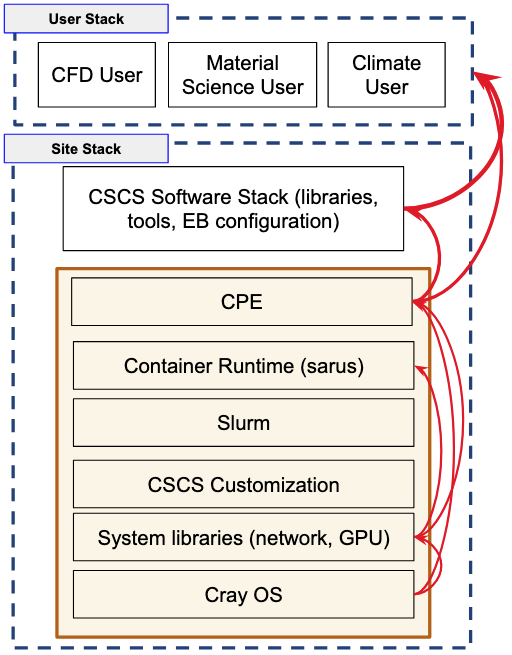
\includegraphics[width=0.3\textwidth]{./images/stack-old.png}
    \end{center}
    \caption{
        The "standard" HPE-EX software stack, with the Cray OS, drivers, CPE and some site software in the system image, site-provided software installed on a shared file system, and software installed by users that depends can depend on different software layers underneath.
        The red arrows indicate where changes on one layer, can have a knock on effect on other software layers, requireing rebuilds or reconfiguration when they are changed.
    }
    \label{fig:stack-old}
\end{figure}

\begin{figure}[htp!]
    \begin{center}
        %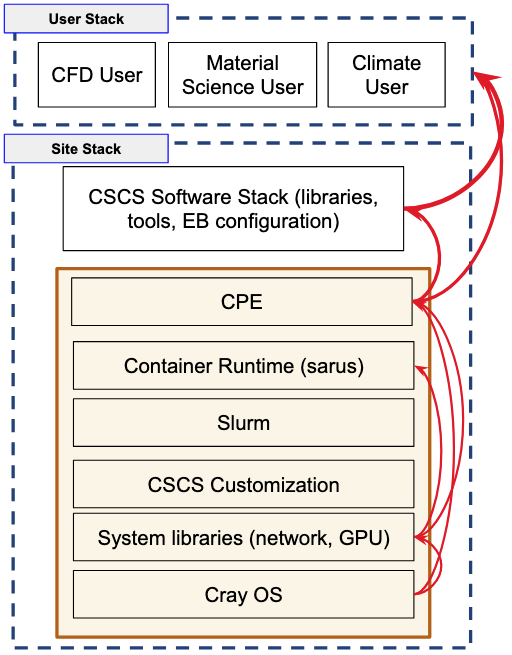
\includegraphics[width=0.3\textwidth]{./images/stack-old.png}
        \todo{image of reduced complexity}
    \end{center}
    \caption{
        The Alps software stack, with the programming environment moved out of the base image.
        Multiple programming environments can be deployed on top of this architecture, including the CPE and alternative PEs discussed in~\sect{sec:spack-stacks} that are mounted at runtime in a new mount namespace by users.
    }
    \label{fig:stack-old}
\end{figure}

The base image is updated less frequently than CPE, so the frequency of rebuilds will be lower than if we built our stack on top of CPE, and the number of system dependencies that could require intervention are fewer.
Furthermore, by providing bespoke environments that contain only the requirements of use case or workflow, we reduce complexity of testing and maintaining PEs.

\todo{Clearly set out the requirements}

\begin{enumerate}
    \item long term stability -- software stack configuration can be maintained for longer
    \begin{itemize}
        \item requirement: reproducable builds
        \item requirement: concise, unambiguous recipes
        \item requirement: minimise system requirements to only the bare minimum (no CPE)
    \end{itemize}
    \item rolling releases and fast fixes -- be able to rebuild and reconfigure at any point
    \item provide use-case or application specific environments (only provide the required minimum)
    \begin{itemize}
        \item requirement: versioning of environments
        \item requirement: fast deployment
    \end{itemize}
    \item deliver a satisfying user experience
    \begin{itemize}
        \item fast configure and build times
        \item compatibility with module, spack, python venv workflows.
    \end{itemize}
\end{enumerate}

CSCS is deploying isolated clusters (vClusters) on the \crayex system called Alps, to provide services to a wider range of user domains, each with their own software, security, reliability and scaling requirements.
The vClusters can be customized for the target use cases, as an alternative to providing one large system with a "one size fits all" programming environment, storage and job scheduler.
This gives CSCS the opportunity to customize the programming environment for vClusters; specifically by providing the smallest possible set of compilers, libraries and tools optimized for the cluster's requirements, node architecture and the Slingshot 11 interconnect.

In this paper we will describe a method for defining, building and deploying alternative programming environments alongside the CPE on \crayex systems.
We provide compact, testable, optimized software environments based on a descriptive recipe that can be updated independently of the CPE release cycle.
The environments are deployed as squashfs images, that users can mount using a SLURM plugin and command line utilities.

